\documentclass[12pt]{article}

\usepackage{graphicx}
\usepackage{longtable}
%\usepackage{hyperref}
\usepackage{verbatim}
\usepackage{tabu}
\usepackage{pdfpages}

\newcommand{\DocumentName}{Software Project Management Plan}
\newcommand{\Title}{\DocumentName \\ \hfill}
\newcommand{\Author}{Lars Van Holsbeeke}
\newcommand{\Version}{1.0}

\begin{document}

\begin{titlepage}

\begin{center}
\includegraphics[width=250pt,angle=90]{../../templates/img/logopdf.pdf}
\vfill
{\Huge \Title}
\hfill
\vfill
\vfill
\end{center}

\begin{minipage}[t]{1\textwidth}
\begin{flushleft}

\includegraphics[width=100pt]{../../templates/img/VUB_logo_compact.jpg}
\end{flushleft}
\end{minipage}

\begin{minipage}[t]{1\textwidth}
\begin{flushright}
\Author \\
\Version \\
\end{flushright}
\end{minipage}

\end{titlepage}


\textbf{Revision History}

\begin{longtable}[c]{@{}lll@{}}
\hline\noalign{\medskip}
Version & Date & Description
\\\noalign{\medskip}
\hline\noalign{\medskip}
\textbf{0.1} & 29/10/2013 & Creation of document structure
\\\noalign{\medskip}
\textbf{0.2} & 03/11/2013 & Completion of initial version
\\\noalign{\medskip}
\textbf{0.3} & 14/11/2013 & Adapted to feedback of initial version
\\\noalign{\medskip}
\textbf{0.4} & 02/12/2013 & Adapted to feedback of version 0.3
\\\noalign{\medskip}
\textbf{1.0} & 12/12/2013 & Updated for delivery, iteration 1
\\\noalign{\medskip}
\hline
\end{longtable}

\begin{center}\rule{3in}{0.4pt}\end{center}

\clearpage

\tableofcontents

\clearpage

\section{Overview}\label{overview}

\subsection{Project Summary}\label{project-summary}

\subsubsection{Purpose, scope, and
objectives}\label{purpose-scope-and-objectives}

The main purpose of this project is to create a working scheduling
webapplication with specific support for mobile devices like smartphones
and tablets that enables (authorized) users to query their personal
course/final schedule and notifies them about last-minute changes. We
will call this application: \texttt{Xiast}\emph{(\textbf{X}iast
\textbf{i}s \textbf{a} \textbf{s}cheduling \textbf{t}ool)} More specific
requirements can be found in the Software
Requirements Specification document.

The main system itself uses the \texttt{Wilma} server of the university
as back-end and a normal or mobile browser as front-end.

All documents, source code and other artifacts are publicly available on
Github. Documents can be found under the \verb=se1-1314/xiast-docs= repository, source code
can be found under \verb=se1-1314/xiast= repository.

This academic 3rth bachelor project is part of the course
``Software Engineering'', taught by dr. R. Van Der
Straeten taking place at the ``Vrije Universiteit Brussel''

\subsubsection{Assumptions and
constraints}\label{assumptions-and-constraints}

Some constraints involving documentation standards, infrastructure and
use of certain technologies have been defined by the client:

\paragraph{Documentation}\label{documentation}

\begin{itemize}
\itemsep1pt\parskip0pt\parsep0pt
\item
  This document (SPMP) must conform the IEEE 1058-1998 standard
\item
  The SRD, SDD, STD, SQAP and SCMP must also conform their IEEE xxx-1998
  standard or a more recent revision of that standard.
\item
  All documents must be written or in Dutch or in English, but not a
  combination of the two.
\item
  All documents must be available in the PDF format
\item
  At least following documents must be maintained:

  \begin{itemize}
  \itemsep1pt\parskip0pt\parsep0pt
  \item
    Software Project Management Plan (SPMP)
  \item
    Software Test Plan (STD)
  \item
    Software Requirements Specification (SRS)
  \item
    Software Design Document (SDD)
  \end{itemize}
\item
  Meeting minutes must be made for all meetings
\item
  An SCMP and an SQMP are not necessary, but all relevant information
  concerning them must be found in the SPMP.
\end{itemize}

\paragraph{Language}\label{language}

\begin{itemize}
\itemsep1pt\parskip0pt\parsep0pt
\item
  Only Clojure, Java, JavaScript, HTML, CSS, SQL and corresponding
  libraries and open-source frameworks
\item
  Only open-source software may be used for both the endproduct and
  tools
\item
  A particular choice of library, tool, etc. must be motivated by means
  of reliabilityn, openness and simplicity.
\item
  A library can only be used after agreement with the client and a
  comparative study of other possible libraries.
\end{itemize}

\paragraph{Infrastucture}\label{infrastucture}

\begin{itemize}
\itemsep1pt\parskip0pt\parsep0pt
\item
  The VUB ``Wilma'' server must be used as backend for
  the system.
\item
  The system must work on a browser as frontend.
\item
  The system must work on a mobile browser.
\end{itemize}

\paragraph{Other Constraints}\label{other-constraints}

\begin{itemize}
\itemsep1pt\parskip0pt\parsep0pt
\item
  ``Github'' must be used as public repository for
  the code.
\item
  All documents, source code and other artefacts must be publicly
  available in a structured way.
\item
  The system must have a standard, easy installation procedure.
\item
  The UI must be simple and attractive to use.
\item
  Requirements IDs may never be renumbered.
\item
  All of the code needs to be documentated.
\item
  Test must be written using the ``JUnit'' framework.
\item
  The system must be modular in design to accomodate extension and
  replacement of the containing modules.
\item
  The development proces must be iterative with incremental delivery.
\end{itemize}

\subsubsection{Project deliverables}\label{project-deliverables}

The table table below shows code, document and other deliverables with
their corresponding deadline: 9 o'clock in the morning on the date
shown.

\begin{longtable}[c]{@{}ll@{}}
\hline\noalign{\medskip}
Date & Deliverable
\\\noalign{\medskip}
\hline\noalign{\medskip}
04/11/2013 & First version of the SPMP
\\\noalign{\medskip}
15/11/2013 & First version of documents
\\\noalign{\medskip}
18/11/2013 & Data dump: data available for use
\\\noalign{\medskip}
13/12/2013 & End of first iteration: delivery of code and documents
\\\noalign{\medskip}
18/12/2013 & First presentation
\\\noalign{\medskip}
04/03/2014 & End of second iteration: delivery of code and documents
\\\noalign{\medskip}
12/03/2014 & Second presentation
\\\noalign{\medskip}
15/04/2014 & End of thirth iteration: delivery of code and documents
\\\noalign{\medskip}
16/05/2014 & End of fourth iteration: final delivery of code and
documents
\\\noalign{\medskip}
21/05/2014 & Final presentation
\\\noalign{\medskip}
\hline
\end{longtable}

\subsubsection{Schedule}\label{schedule}

Section 5.2 describes the work plan of the project, which contains a
detailed description of the work activities with the corresponding
teammembers that work on it along with an estimation of time they will
need to complete it.

\subsection{Evolution of the SPMP}\label{evolution-of-the-spmp}

This SPMP will be reviewed at least one time a week by the
projectmanager. If needed, this document will be updated by the same
person. Each (major) update will be logged in the
Revision History, to be found at the
beginning of this document.

\section{References}\label{references}

\begin{enumerate}
\def\labelenumi{\arabic{enumi}.}
\item
  SRS: Software Requirements Specifiaction

  Anders Deliens\\
  https://github.com/se1-1314/xiast-docs/blob/master/management\\
  /requirements/requirements.md
\item
  Software Engineering course, VUB

  Catalog number: 1004483BNR\\
  https://caliweb.cumulus.vub.ac.be/caliweb/?page=course-offer\&id=001462\\
  \&anchor=2\&target=pr\&year=1314\&language=en\&output=html
\item
  Wilma backend server

  http://wilma.vub.ac.be
\item
  Github

  https://github.com
\item
  JUnit framework

  http://junit.org/
\item
  Markable.in

  Online document writing tool for the Markdown language.
  markable.in
\item
  Iterative and Incremental development model

  Is any combination of both iterative design or iterative method and
  incremental build model for development. For more information:\\
  http://en.wikipedia.org/wiki/Iterative\_and\_incremental\_development
\item
  Agile Software Development

  Topic in the Software Engineering course. Is a group of software
  development methods based on iterative
  and incremental development, where requirements and solutions evolve
  through collaboration between self-organizing, cross-functional teams.
  More information on the course slides or
  http://en.wikipedia.org/wiki/Agile\_software\_development
\item
  Boehm's spiral model

  Is a risk-driven process model generator for software projects.
  Further information: http://en.wikipedia.org/wiki/Spiral\_model
\end{enumerate}

\section{External Stakeholders}\label{external-stakeholders}

\begin{enumerate}
\def\labelenumi{\arabic{enumi}.}
\item
  Ragnhild Van Der Straeten

  Professor of the Software Engineering course. rvdstrae@vub.ac.be
\item
  Jens Nicolay

  Assistant of the Software Engineering course. jens.nicolay@vub.ac.be
\item
  Dirk Van Deun

  System administrator of the Wilma backend server.
  dirk@dinf.vub.ac.be
\end{enumerate}

\section{Definitions}\label{definitions}

\begin{longtable}[c]{@{}ll@{}}
\hline\noalign{\medskip}
Acronym & Declaration
\\\noalign{\medskip}
\hline\noalign{\medskip}
\textbf{DaM} & Database Manager
\\\noalign{\medskip}
\textbf{DeM} & Design Manager
\\\noalign{\medskip}
\textbf{CM} & Configuration Manager
\\\noalign{\medskip}
\textbf{IEEE} & Institute of Electrical and Electronics Engineers
\\\noalign{\medskip}
\textbf{PM} & Project Manager
\\\noalign{\medskip}
\textbf{RM} & Requirements Manager
\\\noalign{\medskip}
\textbf{QAM} & Quality Assurance Manager
\\\noalign{\medskip}
\textbf{SDD} & Software Design Document
\\\noalign{\medskip}
\textbf{SPMP} & Software Project Magement Plan
\\\noalign{\medskip}
\textbf{SRS} & Software Requirements Specification
\\\noalign{\medskip}
\textbf{STD} & Software Test Plan
\\\noalign{\medskip}
\textbf{SQAP} & Software Quality Assurance Plan
\\\noalign{\medskip}
\textbf{SDP} & Software Documentation Plan
\\\noalign{\medskip}
\textbf{VUB} & Vrije Universiteit Brussel
\\\noalign{\medskip}
\textbf{PDF} & Portable Document Format
\\\noalign{\medskip}
\textbf{UI} & User Interface
\\\noalign{\medskip}
IDE & Integrated Development Environment
\\\noalign{\medskip}
\hline
\end{longtable}

Other definitions can be found on page 2-3 of the IEEE 1058-1998
standard for Software Project Management Plans

\section{Project Organisation}\label{project-organisation}

\subsection{External interfaces}\label{external-interfaces}

Client

In this project the titular of this course, Software
Engineering, mrs. R. Van Der Straeten, will together with her
assistant, mr. J Nicolay, act as client for the project. This means that
all communication involving requirements and design will pass by at
least one of them and respectively the
Requirements Manager and the
Design Leader. All other communication with the
client will be handled by the Projectmanager,
this includes submitting deliverables: source-code and documents,
communication involving presentations, etc.

\subsubsection{Infrastructure}\label{infrastructure}

All communication concerning the available infrastructure: the
Wilma backend server will be handled with the head of
infrastructure, mr. D. Van Deun by the web- and databasemanager.

\subsubsection{External Scheduling Data}\label{external-scheduling-data}

Any problems, remarks,\ldots{} involving the dump of scheduling data on
November 18th, 2013 will be communicated to the professor of the course,
mrs. R. Van Der Straeten.

\subsection{Internal Structure}\label{internal-structure}

\subsubsection{Internal Communication}\label{internal-communication}

All communication between the teammembers outside meetings must be
logged by or the issue tracker on Github or using the
internal mailinglist: se1\_1314@wilma.vub.ac.be. This is a rule of thumb
that must be followed by every teammember. Only if the information to
communicate is not important, irrelevant to the other teammembers, does
not involve agreements, deadlines, etc. and the urgency of the
concerning activities is very low, teammembers can use private mail. In
case of urgent problems, problems with another teammember, important
matters that need immediate attention, etc. teammembers may use the
private mobile phone number of the
Projectmanager that has been given to them in
the second meeting.

\subsubsection{Internal Organisation}\label{internal-organisation}

The chart below shows the internal organisation and flows of information
between the actors of the team:

\begin{figure}
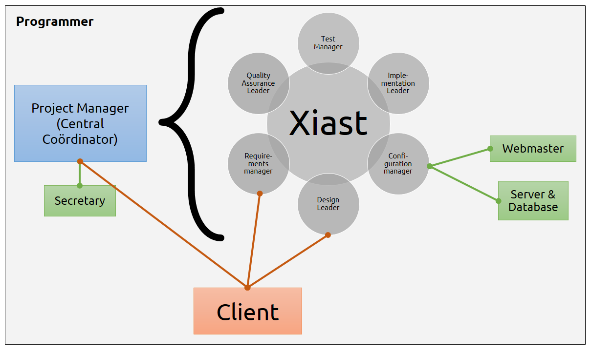
\includegraphics[width=400pt]{organisation.png}
\caption{Internal organisation}
\end{figure}

\begin{itemize}
\itemsep1pt\parskip0pt\parsep0pt
\item
  The Projectmanager acts as a central
  coordination point for the whole team. This means that he is
  responsible to solve (personal) issues between teammembers, He also
  communicates with the client about general project issues concerning
  planning, progress,\ldots{} (see Roles and Responsibilities)
\item
  Every manager has the same grade compared to any other manager. This
  arises from the fact that every teammember fulfills the role of a
  manager, because of the restricted number of teammembers. In this way
  every teammember can communicate problems of any kind to the other
  teammembers without having to propagate them through a complex
  hierarchy of chiefs, leaders, managers, etc. ``Internal
  Communication'' give more information about how this communication
  takes place.
\item
  Because of their (semi) overlap with the tasks of their super
  functions, non-managerial positions (secretary, webmaster and Server
  \& Database manager) will have communicate their issues, reports, etc.
  to their corresponding manager.
\item
  As already mentioned, only the project manager, design leader and
  requirements manager can communicate directly to the client.
\end{itemize}

Roles and Responsibilities

\subsubsection{Main responsibilities}\label{main-responsibilities}

\begin{itemize}
\itemsep1pt\parskip0pt\parsep0pt
\item
  Project Manager

  \begin{itemize}
  \itemsep1pt\parskip0pt\parsep0pt
  \item
    Creating \& providing the SPMP with updates
  \item
    Coordination of the team
  \item
    Contact person for all teammembers
  \item
    Chairman during meetings
  \item
    Creating a weekly meeting agenda on Github
  \item
    Approving decisions taken during meetings
  \item
    Detecting team related problems and solving them
  \item
    Ensuring deadlines are met by all teammembers
  \item
    Ensuring quality of non-code artefacts, created by the teammembers
  \item
    Verifying (together with the secretary) meeting minutes and
    correcting them if needed
  \item
    Creation of a time-scheme, together with the other teammembers
  \item
    Creation of annotated tags on the Github repository (together with
    the configuration manager): one for each iteration
  \item
    Creating presentations
  \end{itemize}
\item
  Configuration Manager

  \begin{itemize}
  \itemsep1pt\parskip0pt\parsep0pt
  \item
    Creating \& providing the SCMP with updates
  \item
    Managing the Github repository for code and
    documents
  \item
    Managing tools used within the team
  \item
    Providing some documentation concerning the used tools and Git.
  \item
    Ensuring safety and restorability of documents
  \end{itemize}
\item
  Quality Assurance Leader

  \begin{itemize}
  \itemsep1pt\parskip0pt\parsep0pt
  \item
    Creation of \& providing the STD with updates
  \item
    Optionally creating (and maintaining) an SQAP
  \item
    Quality-based Monitoring of the Software
  \item
    Reviewing source-code: are all required features implemented?
  \item
    Setting up Unit tests
  \end{itemize}
\item
  Requirements Management Leader

  \begin{itemize}
  \itemsep1pt\parskip0pt\parsep0pt
  \item
    Creation of \& providing the SRS with updates
  \item
    Communicating with client about requirements: p.e. in case of
    ambiguity, special requests, etc.
  \item
    Determines the priority for each working activity
  \item
    Takes care that activities with higher priority are done first
  \item
    Reporting possible changes to the requirements, made by the client
  \end{itemize}
\item
  Design Leader

  \begin{itemize}
  \itemsep1pt\parskip0pt\parsep0pt
  \item
    Creation of \& providing the SDD with updates
  \item
    Determining (and managing) the architecture of the system and
    Database
  \item
    Communicating with the client about the design
  \end{itemize}
\item
  Implementation Leader

  \begin{itemize}
  \itemsep1pt\parskip0pt\parsep0pt
  \item
    Managing of the source code
  \item
    Reporting issues concerning the source code on meetings
  \item
    Distributing programming workload to all teammembers
  \item
    Monitoring developers
  \end{itemize}
\item
  Server \& Database responsible

  \begin{itemize}
  \itemsep1pt\parskip0pt\parsep0pt
  \item
    Regularly updates the website with new information
  \item
    Takes care of communication with the infrastructure manager
  \item
    Manages database, server applications and related services
  \end{itemize}
\item
  Webmaster

  \begin{itemize}
  \itemsep1pt\parskip0pt\parsep0pt
  \item
    Maintains the static website, generated by GitHub pages
  \item
    Maintains the project website on which Xiast runs
  \end{itemize}
\item
  Secretary

  \begin{itemize}
  \itemsep1pt\parskip0pt\parsep0pt
  \item
    Creates meeting minutes during meetings
  \item
    Maintains and corrects this minutes after eacht meeting
  \end{itemize}
\end{itemize}

\subsubsection{Documentation
responsibilities}\label{documentation-responsibilities}

\begin{longtable}[c]{@{}ll@{}}
\hline\noalign{\medskip}
Responsible teammember & Document(s)
\\\noalign{\medskip}
\hline\noalign{\medskip}
Youssef Boudiba & STD, SQAP
\\\noalign{\medskip}
Anders Deliens & SRS
\\\noalign{\medskip}
Adriaan Leijnse & SDD
\\\noalign{\medskip}
Kwinten Pardon & SDP
\\\noalign{\medskip}
Nils Van Geele & SCMP
\\\noalign{\medskip}
Lars Van Holsbeeke & SPMP
\\\noalign{\medskip}
\hline
\end{longtable}

\section{Managerial Process Plans}\label{managerial-process-plans}

\subsection{Start-up Plan}\label{start-up-plan}

\subsubsection{Staffing Plan}\label{staffing-plan}

 H = Function Holder, B = Back-up

%\begin{longtable}[c]{@{}lcccccc@{}}
\begin{longtabu}[c]{@{}lXXXXXX@{}}
\hline\noalign{\medskip}
Function/Teammember & Youssef Boudiba & Anders Deliens & Adriaan Leijnse
& Kwinten Pardon & Nils Van Geele & Lars Van Holsbeeke
\\\noalign{\medskip}
\hline\noalign{\medskip}
Project Manager & & B & & & & H
\\\noalign{\medskip}
Configuration Manager & & & & & H & B
\\\noalign{\medskip}
Quality Assurance Leader & H & & & B &
\\\noalign{\medskip}
Requirements Manager & & H & B & &
\\\noalign{\medskip}
Design Leader & & & H & & B
\\\noalign{\medskip}
Implementation Leader & B & & & H &
\\\noalign{\medskip}
Secretary & & B & & & H
\\\noalign{\medskip}
Server \& Database & & & B & & H
\\\noalign{\medskip}
Test Manager & H & & & B &
\\\noalign{\medskip}
Webmaster & & & & & H & B
\\\noalign{\medskip}
\hline
\end{longtabu}
%\end{longtable}

\subsubsection{Project Staff Training
Plan}\label{project-staff-training-plan}

Each teammembers is responsible to become familiar with the
technologies, languages, etc. used in the project. It is therefore
highly recommended to use information from books, (online) tutorials,
other teammembers, etc. to resolve the lack of any foreknowledge. At the
beginning of the project, the situation is as follows

\begin{itemize}
\itemsep1pt\parskip0pt\parsep0pt
\item
  Youssef: Has experience with Java and Git but hasn't any experience
  with Clojure, Latex and webtechnologies
\item
  Anders: Has programming skills and lots of experience with group
  projects and LaTeX, but never used Git and Clojure before
\item
  Adriaan: Has lots of experience with Git, Clojure and LaTex but less
  with webtechnologies
\item
  Kwinten: Is very experienced with webtechnologies, has lots of
  experience with Git, less with LaTex and none with Clojure
\item
  Nils: Has lots of experience with Git, LateX and webtechnologies, but
  less with Clojure
\item
  Lars: Has experience with Java and LateX, less with Git and
  webtechnologies and none with Clojure.
\end{itemize}

Based on this information it would be very useful for teammembers to
follow tutorials concerning the technologies/languages they are not
familiar with. This leads to the following situation: \emph{XX = highly
recommended, X = recommended, V = not really necessary}

\begin{longtable}[c]{@{}lcccccc@{}}
\hline\noalign{\medskip}
Training & Youssef & Anders & Adriaan & Kwinten & Nils & Lars
\\\noalign{\medskip}
\hline\noalign{\medskip}
Clojure & XX & XX & V & XX & X & XX
\\\noalign{\medskip}
LaTeX & X & V & V & V & V & V
\\\noalign{\medskip}
Git & X & XX & V & V & V & XX
\\\noalign{\medskip}
Webtechnologies & XX & XX & X & V & X & X
\\\noalign{\medskip}
\hline
\end{longtable}

\subsection{Work Plan}\label{work-plan}

\subsubsection{Work activities}\label{work-activities}

The table below shows an overview of the different activities in the
development process together with the responsible teammember and an
estimation of time needed to complete the activity. Rough time
estimations were made by the group and are based on the total workload
of each package of activities concerning this iteration (iteration 1).
This way of estimation has been chosen because the models
(Albrecht/IFPUG, Symons/Mark,COSMIC,COCOMO8I, COCOMOII, \ldots{}) are
made for business software development in the real world (with a real
company). We are only students simulating a software company, we don't
have the amount of rescources, infrastructure,\ldots{} a real company
has. In this way these models would lead to untrustworthy
(time)estimations.

\subsubsection{Planning per iteration}\label{planning-per-iteration}

\begin{itemize}
\itemsep1pt\parskip0pt\parsep0pt
\item
  \textbf{Iteration 1 ``Writing web applications in Clojure''},
  \emph{December 13th, 2013}

  \begin{itemize}
  \itemsep1pt\parskip0pt\parsep0pt
  \item
    Interfaces: A single web interface using dynamically generated
    static web pages is used.

    \begin{itemize}
    \itemsep1pt\parskip0pt\parsep0pt
    \item
      Internationalisation: The interface needs to be displayed in both
      English and Dutch, depending on user preference.
    \end{itemize}
  \item
    Logging in: Using the VUB's authentication API.
  \item
    Courses: Viewing a list of courses, optionally filtered through a
    keyword.
  \item
    Schedules: Viewing the entire schedule of a course, logged in
    student or room.
  \end{itemize}
\item
  \textbf{Iteration 2 ``Making Clojure and JavaScript work together''},
  \emph{March 4th, 2014}

  \begin{itemize}
  \itemsep1pt\parskip0pt\parsep0pt
  \item
    Interfaces: Both a mobile and a desktop interface need to be
    provided.
  \item
    Schedules for whole programs
  \item
    Permission system: Program managers can only change the courses they
    own, etc.
  \item
    Configuration file driven scheduling algorithm: To make a simple
    start without introducing too much complexity in the front-end.
  \item
    Program managers can add programs through a web-interface
  \item
    Program managers can add rooms through a web-interface
  \item
    Instructors can change course details of existing courses: E.g.
    ``this course requires an overhead projector'', etc.
  \end{itemize}
\item
  \textbf{Iteration 3 ``Full base functionality''}, \emph{April 15th,
  2014}

  \begin{itemize}
  \itemsep1pt\parskip0pt\parsep0pt
  \item
    Web interface for program manager business: Scheduling courses,
    configuring programs, etc.
  \item
    Messaging system for schedule suggestions: Instructors and program
    managers need to communicate/request schedule changes. These should
    be easily appliable to the actual schedule by a program manager.
  \end{itemize}
\item
  \textbf{Iteration 4 ``Extra features and polishing up''}, \emph{May
  16th, 2014}

  \begin{itemize}
  \itemsep1pt\parskip0pt\parsep0pt
  \item
    E-mail notifications for students about schedule changes
  \end{itemize}
\end{itemize}

\paragraph{Time estimations}\label{time-estimations}

Time estimations are made in hours (h).

\subparagraph{Iteration 1}\label{iteration-1}

\begin{longtable}[c]{@{}llrl@{}}
\hline\noalign{\medskip}
Activity & Responsible & Est. Time & Documents
\\\noalign{\medskip}
\hline\noalign{\medskip}
Quality Checks & QAM & 5 & (SQAP)
\\\noalign{\medskip}
Tests & QAM & 15 & STD
\\\noalign{\medskip}
Requirements management & RM & 35 & SRS
\\\noalign{\medskip}
Design & DeM & 20 & SDD
\\\noalign{\medskip}
Implementation & IL, programmers & 50 & source code
\\\noalign{\medskip}
Configuration management & CM & 30 & SCMP
\\\noalign{\medskip}
Team management & PM & 60 & SPMP
\\\noalign{\medskip}
Training & n.a. & 30 & n.a.
\\\noalign{\medskip}
\hline
\end{longtable}

\paragraph{Actual performed time}\label{actual-performed-time}

During the development proces, each teammember will log how much time he
spends on an activity of the project. This includes time spend on
programming, documentation, testing, versioning control, etc. but also
time spend on meetings. At every (weekly) meeting, each team member
should tell how much time he has spent on which activity.

Performed time has been logged in hours (h). 

\begin{longtable}[c]{@{}llrl@{}}
\hline\noalign{\medskip}
Teammember & Function & Perf. Time & Documents
\\\noalign{\medskip}
\hline\noalign{\medskip}
Youssef Boudiba & QAM & 27 & STD, (SQAP)
\\\noalign{\medskip}
Anders Deliens & RM & 31 & SRS
\\\noalign{\medskip}
Adriaan Leijnse & DeM & 52 & SDD
\\\noalign{\medskip}
Kwinten Pardon & IL, programmers & 44 & source code
\\\noalign{\medskip}
Nils Van Geele & CM & 44 & SCMP
\\\noalign{\medskip}
Lars Van Holsbeeke & PM & 67 & SPMP
\\\noalign{\medskip}
\hline
\end{longtable}

\emph{TOTAL: 265 hours}

\subsubsection{Schedule allocation}\label{schedule-allocation}

A GANTT chart is used for this. The major part of the activities depends
on the release of the SRS, because the latter contains all requirements
on which our project is build. The majority of the dependencies between
activities are logically derivable from the GANTT-chart.

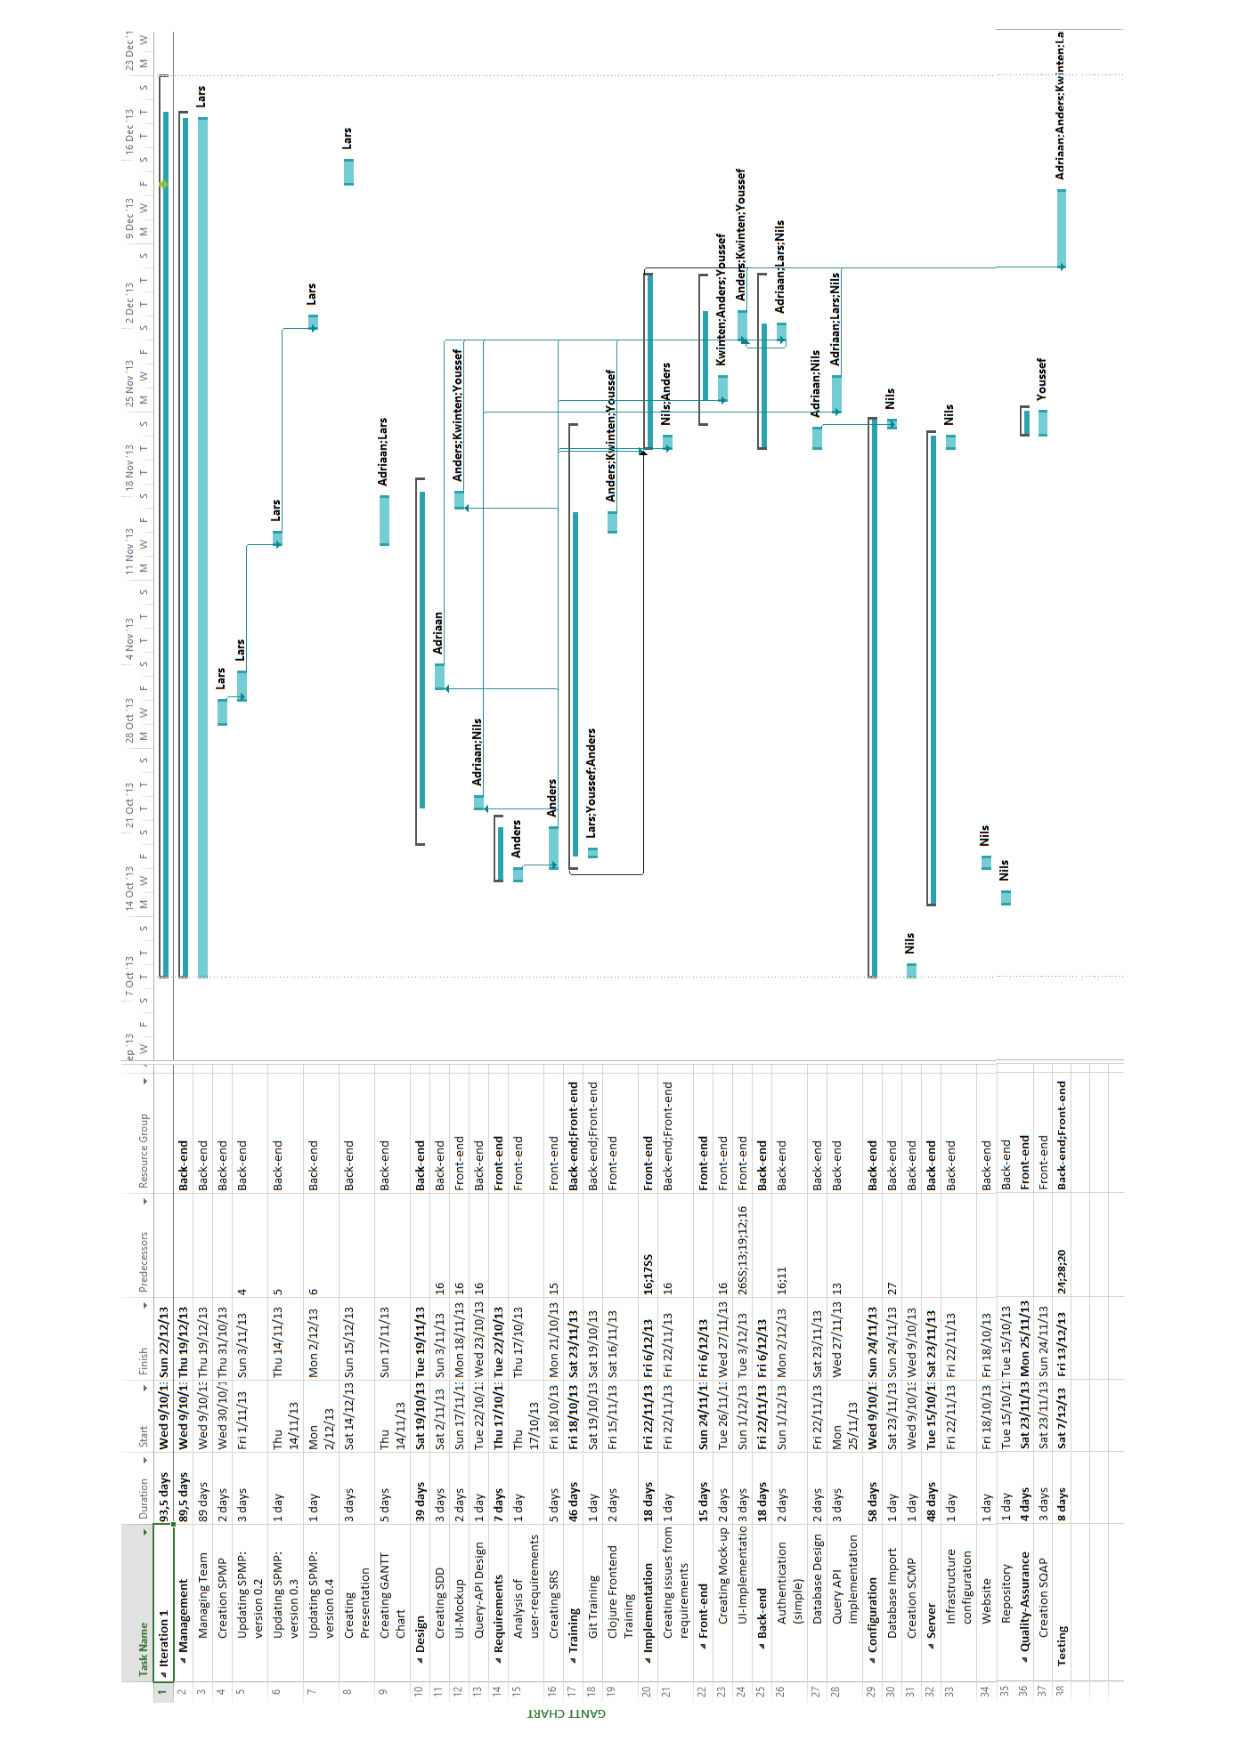
\includepdf[pages={1}]{gannt_iter1.pdf}
%\begin{figure}[hbtp]
%	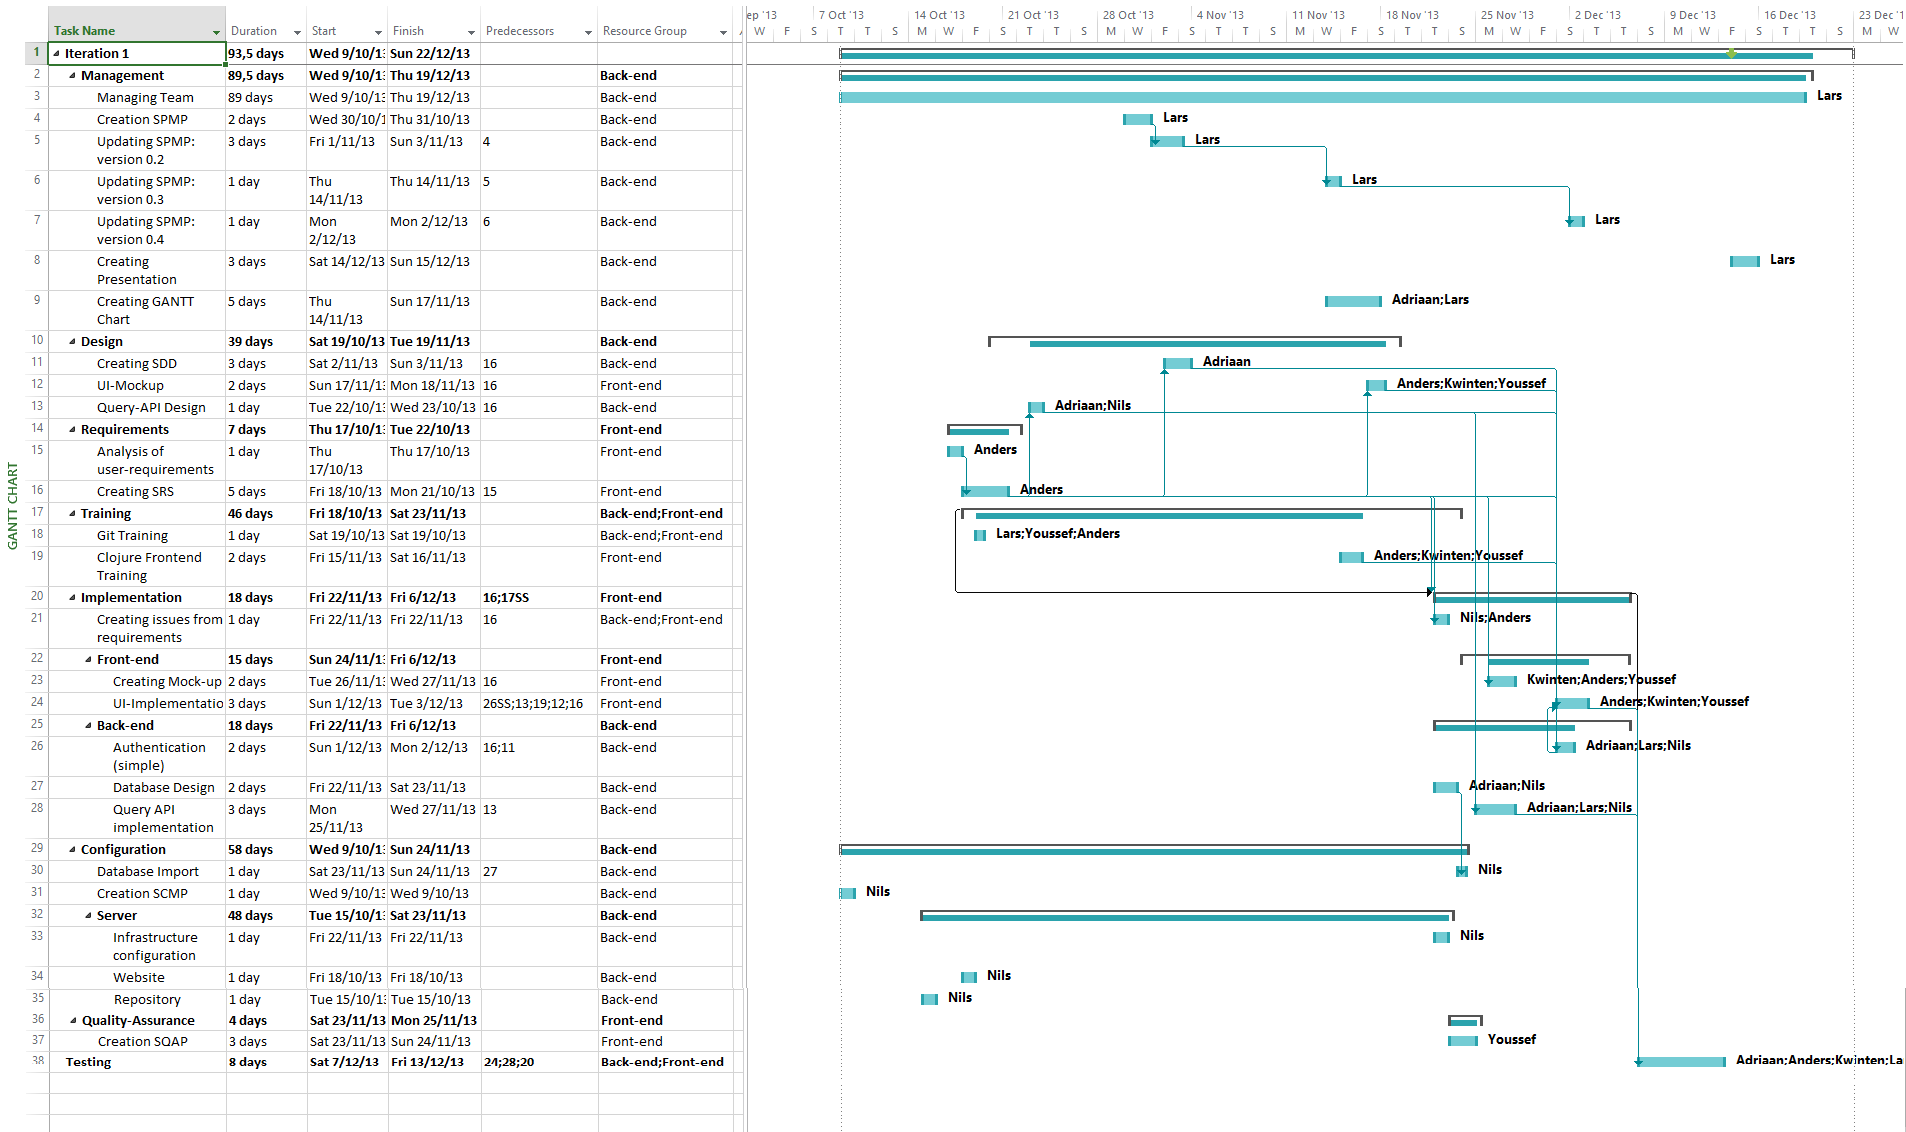
\includegraphics[width=750pt,keepaspectratio,angle=90]{GANNT_Iter1.PNG}
%	\caption{GANNT chart for iteration 1}
%\end{figure}

\subsubsection{Resource allocation}\label{resource-allocation}

An overview of rescources that will be used can be found in the table
below

\begin{longtable}[c]{@{}ll@{}}
\hline\noalign{\medskip}
Rescource & Activities
\\\noalign{\medskip}
\hline\noalign{\medskip}
Wilma backend server & Application backend; Hosting of
the static website
\\\noalign{\medskip}
Microsoft Project & Project Management (tool)
\\\noalign{\medskip}
Microsoft PowerPoint & Presentations
\\\noalign{\medskip}
Markable & Writing documents in the Markdown
language
\\\noalign{\medskip}
Github & Versioning Control System
\\\noalign{\medskip}
Smartphone (Android) & Testing mobile version of the tool
\\\noalign{\medskip}
\hline
\end{longtable}

\subsection{Control Plan}\label{control-plan}

\subsubsection{Requirements control
plan}\label{requirements-control-plan}

Possible changes of requirements will always be communicated between the
requirements manager and the client. When a change occurs, the
requirements manager puts an new topic on the agenda of the next
teammeeting and updates the SRS.

\subsubsection{Schedule control plan}\label{schedule-control-plan}

Problems involving scheduling, deadlines, etc. will be discussed during
the weekly meeting. Each teammember is responsible to keep track of his
deadlines, and will report (at the weekly meeting) what he has done on
which activity during the last week. The projectmanager himself will
keep track of the global planning by using these reports and make
adjustments to the planning and/or activity if needed. If it seems that
one of the teammembers won't make the deadline, one or more other
teammembers can jump in on the activity concerned. This is highly
appreciated.

\subsubsection{Quality control plan}\label{quality-control-plan}

All code and documentation will be periodically checked by the Quality
Assurance Manager and before the end of each iteration. First he reports
(if needed) to the concerning person. If any severe (quality based)
problems are detected, he will report also them at the weekly meeting.

\subsubsection{Reporting plan}\label{reporting-plan}

Using the SPMP, SCMP, STD and SDD, the status of the project will be
reported to external entities (p.e. the client). All this documents are
free to be read by anybody on our Github repository.
It can be reached and downloaded by using our
static website on
http://wilma.vub.ac.be/\textasciitilde{}se1\_1314

\subsection{Risk management plan}\label{risk-management-plan}

This list will be extended in future versions of this document All
estimations are on a scale from 0 to 10.

\begin{enumerate}
\def\labelenumi{\arabic{enumi}.}
\itemsep1pt\parskip0pt\parsep0pt
\item
  One of the teammembers is sick or leaves

  \begin{itemize}
  \itemsep1pt\parskip0pt\parsep0pt
  \item
    Probability: medium
  \item
    Impact: high
  \item
    Priority: high
  \item
    Cost of solution: high
  \item
    Solution: Teammember with corresponding back-up function takes over.
  \item
    Target completion date: n.a.
  \item
    Responsible: Project Manager
  \end{itemize}
\item
  Bad communication between teammembers

  \begin{itemize}
  \itemsep1pt\parskip0pt\parsep0pt
  \item
    Probability: medium
  \item
    Impact: medium
  \item
    Priority: high
  \item
    Cost of solution: low
  \item
    Solution: Don't use too much private communication, use the
    mailinglist. The issue tracker on Github must be
    up-to-date at all times.
  \item
    Target completion date: n.a.
  \item
    Responsible: Project Manager
  \end{itemize}
\item
  Not meeting deadlines

  \begin{itemize}
  \itemsep1pt\parskip0pt\parsep0pt
  \item
    Probability: medium
  \item
    Impact: high
  \item
    Priority: high
  \item
    Cost of solution: low
  \item
    Solution: Keeping track of progress made using
    Github functionality, weekly progress reports of
    teammembers.
  \item
    Target completion date: n.a.
  \item
    Responsible: Project Manager
  \end{itemize}
\item
  Lack of software quality

  \begin{itemize}
  \itemsep1pt\parskip0pt\parsep0pt
  \item
    Probability: low
  \item
    Impact: low
  \item
    Priority: low
  \item
    Cost of solution: medium
  \item
    Solution: Periodically quality checks, tests,\ldots{} Reporting them
    to the weekly meeting. QAM gives recommendations to the teammembers
    on the weekly meeting and by using the mailing list. Making and
    resolving issues on the Github issue tracker.
  \item
    Target completion date: n.a.
  \item
    Responsible: Quality Assurance Manager
  \end{itemize}
\item
  Misunderstandings between client and team

  \begin{itemize}
  \itemsep1pt\parskip0pt\parsep0pt
  \item
    Probability: low
  \item
    Impact: high
  \item
    Priority: high
  \item
    Cost of solution: medium
  \item
    Solution: Regular meetings with the client to check if product meets
    expectations
  \item
    Target completion date: n.a.
  \item
    Responsible: Requirements Manager
  \end{itemize}
\item
  Conflicts between teammembers

  \begin{itemize}
  \itemsep1pt\parskip0pt\parsep0pt
  \item
    Probability: low
  \item
    Impact: high
  \item
    Priority: high
  \item
    Cost of solution: high
  \item
    Solution: Negotiation between the teammembers involved, together
    with the projectmanager.
  \item
    Target completion date: n.a.
  \item
    Responsible: Project Manager
  \end{itemize}
\item
  Abrupt changes in requirements

  \begin{itemize}
  \itemsep1pt\parskip0pt\parsep0pt
  \item
    Probability: low
  \item
    Impact: high
  \item
    Priority: high
  \item
    Cost of solution: medium (depends)
  \item
    Solution: Using the modularity of the software product to implement
    as easily and efficiently as possible the changes. Prevention by
    involving the client in the development process.
  \item
    Target completion date: n.a.
  \item
    Responsible: Requirements manager, Implementation Leader
  \end{itemize}
\item
  Wrong interpretation of requirements by the team

  \begin{itemize}
  \itemsep1pt\parskip0pt\parsep0pt
  \item
    Probability: medium
  \item
    Impact: high
  \item
    Priority: high
  \item
    Cost of Solution: medium (depends)
  \item
    Solution: Using the modularity of the software product to correct as
    easily and efficiently as possible the requirements that were
    misunderstood
  \item
    Target completion date: n.a.
  \item
    Responsible: Requirements Manager, Implementation Leader
  \end{itemize}
\item
  Apache server goes offline on Wilma

  \begin{itemize}
  \itemsep1pt\parskip0pt\parsep0pt
  \item
    Probability: low
  \item
    Impact: medium
  \item
    Priority: high
  \item
    Cost of Solution: low
  \item
    Solution: Changing the url in the configuration of the application
  \item
    Target completion date: n.a.
  \item
    Responsible: Server Manager
  \end{itemize}
\item
  Database server goes offline

  \begin{itemize}
  \itemsep1pt\parskip0pt\parsep0pt
  \item
    Probability: low
  \item
    Impact: high
  \item
    Priority: high
  \item
    Cost of Solution: low
  \item
    Solution: Changing the configuration of the application (dataloss of
    a part of the database is possible). The cost of this solution is
    low because back-ups of the database are taken every hour, using a
    back-upserver of a teammember
  \item
    Target completion date: n.a.
  \item
    Responsible: Server Manager
  \end{itemize}
\item
  Back-end server goes (temporarly) down

  \begin{itemize}
  \itemsep1pt\parskip0pt\parsep0pt
  \item
    Probability: low
  \item
    Impact: high
  \item
    Priority: high
  \item
    Cost of solution: low
  \item
    Solution: Using a mirror server: Aphrodite
  \item
    Target completion date: n.a.
  \item
    Responsible: Server Manager
  \end{itemize}
\end{enumerate}

\subsection{Closeout plan}\label{closeout-plan}

Not of any importance to this project.

\section{Technical Process Plan}\label{technical-process-plan}

\subsection{Process model}\label{process-model}

We will be using the Iterative and
Incremental development model with some ideas of
Agile Software Development, which is based on this
model. This method has been chosen firstly because of the agenda of the
project which consists of an incremental delivery based on four
iterations. Secondly, it has been chosen for its simplicity and added
value: we focus on a working application per iteration which can than be
discussed with the client. In this way we open ourselves up to
requirements changes which will be given to us by the client at the end
of each iteration. This results in a continuous delivery of valuable
software, one of the key principles of agile development. The figure
below shows (Boehm's) spiral model, which will
be used as development process model.

\begin{itemize}
\itemsep1pt\parskip0pt\parsep0pt
\item
  One iteration consists of four phases:

  \begin{itemize}
  \itemsep1pt\parskip0pt\parsep0pt
  \item
    Determination of objectives: In this phase changes in requirements
    will be determined and introduced in the SRS\\
  \item
    Identification (and resolving) risks: This phase involves the
    identification of possible risks caused by changed requirements:
    these will be discussed in the weekly meetings
  \item
    Developing and testing: Using the changed/extended design of the
    previous iteration, new and changed functionality will be
    implemented by the developers. The coordination of this phase is
    being done by the implementation leader, software quality assurance
    manager, design manager and test manager
  \item
    Planning of the next iteration: Releasing the new version of the
    product is the first thing to be done in this iteration. After this,
    the next iteration will be planned by the project manager.
  \end{itemize}
\end{itemize}

\begin{figure}
	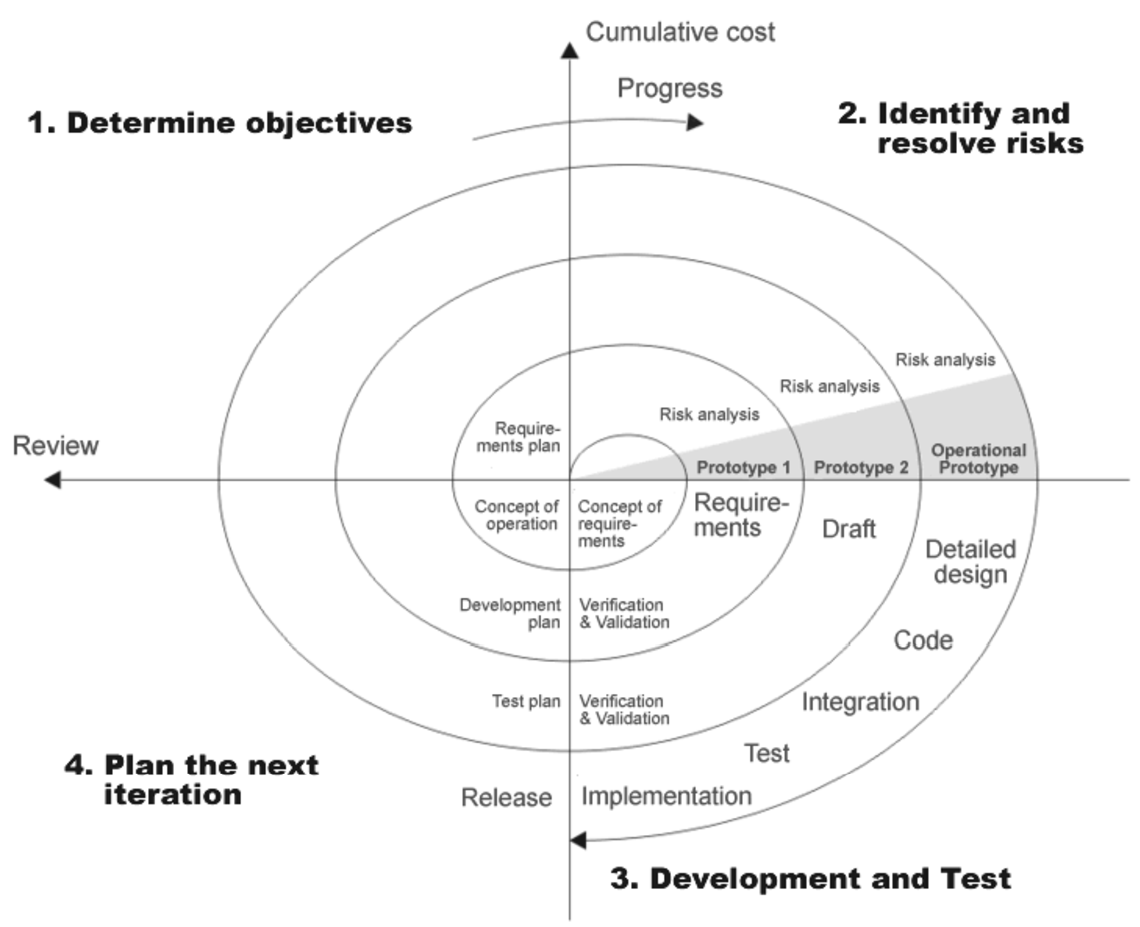
\includegraphics[width=350pt]{BoehmSpiral.pdf}
	\caption{Boehm's Spiral}
\end{figure}

\subsection{Methods, tools and
techniques}\label{methods-tools-and-techniques}

\begin{itemize}
\itemsep1pt\parskip0pt\parsep0pt
\item
  Github will be used as

  \begin{itemize}
  \itemsep1pt\parskip0pt\parsep0pt
  \item
    communication tool for documents
  \item
    versioning control system for source code
  \end{itemize}
\item
  Clojure will be used as programming language

  \begin{itemize}
  \itemsep1pt\parskip0pt\parsep0pt
  \item
    Back-end: to generate schedules and provide an API to login/logout
    and to view and modify schedules
  \item
    Front-end: to query schedules using the back-end api.
  \end{itemize}
\item
  JavaScript and JQuery to create dynamic webpages, used to view/update
\item
  Every teammember is free to use his preferred IDE during the
  implementation process
\item
  A MySQL database will be used as backend database on Wilma. It will be
  populated with course schedule data.
\item
  Markdown will be used to write documents because of its perfect
  integration with Github. When documents must be delivered, Pandoc will
  be used to convert the Markdown documents to the `paper-compatible'
  LaTeX language from which pdf files are generated.
\item
  Compojure and Ring are used as the main webframeworks for Clojure.
\end{itemize}

\section{Supporting Process Plans}\label{supporting-process-plans}

\subsection{Software Configuration Management Plan
(SCMP)}\label{software-configuration-management-plan-scmp}

\subsubsection{Introduction}\label{introduction}

In this document we will describe the workflow that needs to be followed
for the Xiast project. We will also talk about the two \textbf{Git}
repositories that will be used. This document will also be included in
an adapted form in the SPMP.

\subsubsection{The repositories}\label{the-repositories}

For this project we will be using two distinct Git repositories, each
with their own specific purpose.

\paragraph{xiast-docs}\label{xiast-docs}

The \texttt{xiast-docs} repository will be used to hold all documents
related to the project. This includes reports made during meetings and
all plans made by the different leaders and managers.

Every manager has his own directory inside the \texttt{management}
directory. In this directory, the manager can put all files related to
his work and reports. If a manager wants to make a change to the main
directory structure, he is free to do so but must contact the
configuration manager about it. By doing this the software configuration
manager can keep the directory structure in the SCMP up-to-date.

The current directory structure, which may be subject to change, is:

\begin{itemize}
\itemsep1pt\parskip0pt\parsep0pt
\item
  \textbf{/}

  \begin{itemize}
  \itemsep1pt\parskip0pt\parsep0pt
  \item
    \textbf{management} directory containing all official documentation

    \begin{itemize}
    \itemsep1pt\parskip0pt\parsep0pt
    \item
      \textbf{configuration} concerning project configuration
    \item
      \textbf{design} concerning software design
    \item
      \textbf{implementation} concerning implementation
    \item
      \textbf{project} concerning project planning and management
    \item
      \textbf{quality} concerning software quality and testing
    \item
      \textbf{requirements} concerning all software requirements
    \end{itemize}
  \item
    \textbf{meetings} contains all agendas and reports of meetings
  \item
    \textbf{manuals} contains all files related to the Xiast manuals
  \item
    \textbf{templates} contains templates for deliverables
  \end{itemize}
\end{itemize}

\paragraph{xiast}\label{xiast}

The \texttt{xiast} repository is the main repository that contains all
the code for both the server and the Xiast website. The directory
structure is that of a basic Leiningen project:

\begin{itemize}
\itemsep1pt\parskip0pt\parsep0pt
\item
  \textbf{/}

  \begin{itemize}
  \itemsep1pt\parskip0pt\parsep0pt
  \item
    \textbf{resources}

    \begin{itemize}
    \itemsep1pt\parskip0pt\parsep0pt
    \item
      \textbf{dictionaries} directory containing translates strings for
      internationalisation
    \item
      \textbf{public} directory containing public files such as images,
      CSS stylesheets, \ldots{}
    \item
      \textbf{templates} directory containing all website templates
    \end{itemize}
  \item
    \textbf{src} directory containing the source files
  \item
    \textbf{test} directory containing all tests
  \end{itemize}
\end{itemize}

The \texttt{xiast} repository is for code and related resources
(graphics, sound, SQL, \ldots{}) only.

\subsubsection{Tracking issues}\label{tracking-issues}

With GitHub's issue tracker, which can be found here\footnote{https://github.com/se1-1314/xiast/issues}, we can create
so-called \emph{issues}. An issue can be anything from a bug, request
for implementation or suggestion, goal, \ldots{} By using this tool we
can achieve a workflow that will make it easier for both us and others
to track the progress of the project.

When all requirements of the project are known, we will start splitting
up the requirements in one or more smaller ``tasks'' that need to be
finished in order to implement the requirement. These issues can then be
bundled into a \emph{milestone} which denotes the requirement or part of
the requirement that needs to be implemented. Milestones feature
progress trackers which again makes it really easy for people to see how
much still needs to be done for a requirement.

For example: ``Functioning user system'' can be a milestone, with issues
such as ``User registration'' and ``User login'', or ``Access control''
with ``Assigning user rights'' and ``Rights checking'' as some of the
issues.

As mentioned earlier, the issue tracker can and must be used for more
than just tracking progress of the requirements. Issues will be made to
report bugs and propose fixes, to propose enhancements or request extra
functionality, to report on critical errors and so on. Every issue
features a comment section which makes it easy for team members to
discuss requests, bugs, and so on.

It is important that the issue tracker is kept clean at all times. What
this means is that all issues and milestones have proper descriptions
and descriptive titles, issues that are finished must be closed (see
workflow), when one team member takes over an issue from another team
member this must be updated on the tracker, \ldots{} and so on.

The usage of the issue tracker, when done properly, causes less overhead
on the project because we do not need to maintain our own tracker or
website.

\subsubsection{Git workflow}\label{git-workflow}

When working with Git, there are multiple workflows possible.
Considiring the size of the team and project, we will be using the so
called \textbf{feature branching workflow}. This workflow allows us to
tightly integrate the issue tracker into our project.

\paragraph{Branches}\label{branches}

There will always be one central branch: the \textbf{master} branch.
This branch is the actual ``master copy'' of our project and should
contain preferably only working code.

Whenever a team member wants to implement changes, he must first branch
the master branch into a new one and commit all his changes to the newly
created branch. This branch, which is created locally, needs to be
published to GitHub. This doesn't only make it easier to track changes
on the branch, but also makes it easier to transfer the work to someone
else.

Because some issues have a really small workload and can be solved in a
single commit, it's possible to solve multiple issues on one single
branch instead of creating a branch for every issue.

To keep things uniform, branch names must be in lower case only and use
dashes instead of spaces.

\paragraph{Merging}\label{merging}

After the work has been done and the issue is implemented, the working
branch needs to be merged into the \texttt{master} branch. It is mainly
the team member's responsibility to avoid merge conflicts!

Conflicts can be avoided more easily by periodically pulling and merging
the \texttt{master} branch into the working branch, and not vice versa.
By doing this regulary, conflicts that will occur will be smaller than
they would be if we didn't merge at all.

If and only if all work is done and the working branch is conflict free
and the head of the branch is pushed to GitHub, steps can be taken to
merge the working branch into the \texttt{master} branch. This is done
by making a \textbf{pull request}.

\paragraph{Pull request}\label{pull-request}

When making a pull request, select the \texttt{master} branch as the
base branch and the working branch as the compare branch. If the branch
that is being merged closes one or more issues, they should be
referenced in the description. If done correctly, like described in
this
guide\footnote{https://help.github.com/articles/closing-issues-via-commit-messages}, the issues can be automatically closed when the pull request
gets accepted.

After making the pull request, it is the (backup) implementation
manager's responsibility to accept or deny the request. The first step
is to review the code by testing it locally to see if it actually works.
If he so chooses, he can also simulate the merging locally to see if it
works with previous accepted pull requests.

If the code works and there are no conflicts, the pull request can be
accepted and close. After this, the appropriate issue should be closed
too and a comment with a link to the pull request should be made. To
avoid ``branch pollution'' the working branch can safely be removed from
the repository by GitHub after accepting the pull request.

If conflicts arise during merging because of for instance earlier
accepted pull requests, the implementation manager can choose to fix the
conflicts himself manually or just denying and closing the pull request.
The second option is advised. In this case, the team member must fix his
code and make a new pull request. The same is valid for when there are
problems with the code itself.

\paragraph{Assigning and reassigning
issues}\label{assigning-and-reassigning-issues}

To keep track of who is working on what and to avoid double work,
members should assign themselves or others to issues. This can be done
on the issue tracker itself.

If a team member is stuck, the member is free to transfer the work to
someone else. But he must not forget to reassign the issue to the other
person

\paragraph{docs}\label{docs}

For the \texttt{xiast-docs} repository, we don't need to use the feature
branch workflow, we can just use a \textbf{centralized workflow}. This
means we won't use branching and we will just commit to the master
branch.

\subsubsection{Project website}\label{project-website}

One of the requirements of the project is a website that can be used to
track the progress of the project. Instead of focussing on implementing
our own system, we will make full use of the tools GitHub is providing
us.

The website can be reached at \texttt{http://se1-1314.github.io/xiast}.
This page, which is generated using GitHub Pages, contains information
about the project, including download links for the source code and
links to various documents.

GitHub Pages is in essence a static website generator. This means that,
given the contents of the site, it only needs to generate all the HTML
and related files once. This not only makes it faster, but also a lot
easier.

The automatic page generator can be found on the settings page of the
project. The files it generates are located in the \texttt{gh-pages}
branch of the \texttt{xiast} repository. Commiting to this branch thus
allows us to edit the page manually, although it is highly advised to
keep using the automatic page generator and edit the content of the site
using markdown.

To keep track of the project's status however, we will use the built-in
issue tracker of GitHub.

\subsection{Software Quality Assurance Plan
(SQAP)}\label{software-quality-assurance-plan-sqap}

The Software Quality Assurance Plan (SQAP) is based on the IEEE standard
for software quality assurance plans (730-2002). Since almost all
information can be found in the SPMP, we will not cover every topics
proposed by the standard.

\subsubsection{Purpose}\label{purpose}

This SQAP's objective is to ensure that the project does not deviate
from its requirements and that a certain level of quality is maintained.
By defining several methods and guidelines we ensure that the
development of the project proceeds smoothly while keeping the quality
high.

\subsubsection{Tasks}\label{tasks}

The main tasks of the QAM consist of:

\begin{itemize}
\itemsep1pt\parskip0pt\parsep0pt
\item
  Writing and updating of the SQAP.
\item
  Writing and updating of the STD.
\item
  Checking whether or not the delivered documents confirm to their
  purpose.
\item
  Checking if all documents are consistent and follows established
  guidelines (coding style, use of template for all documents, etc.).
\end{itemize}

\subsubsection{Standards, practices, conventions and
metrics}\label{standards-practices-conventions-and-metrics}

\paragraph{Documentation Standards}\label{documentation-standards}

All documents must be based on IEEE standards and follow a certain
template.

All documentation and source code must be written in English (except
meetings reports that will be written in Dutch).

\paragraph{Coding (and comment)
Standards}\label{coding-and-comment-standards}

The code documentation must follow the SDP.

\paragraph{Testing standards}\label{testing-standards}

Testing of code must follow steps of to the STD.

\paragraph{Metrics}\label{metrics}

During random checks, the quality of the project will be measured by
using following metrics:

\begin{itemize}
\itemsep1pt\parskip0pt\parsep0pt
\item
  Test Pass Rate.
\item
  Numbers of bugs found per tests.
\item
  Time to fix bug/close issue.
\end{itemize}

Exact numbers will be communicated later.

\paragraph{Conventions}\label{conventions}

We'll organize weekly meetings to resume the current state of the
project and to discuss the evolution of it.

\subsubsection{Test}\label{test}

All the information about testing methodology, procedures and execution
can be found in the STD.

\subsubsection{Problem reporting and corrective
actions}\label{problem-reporting-and-corrective-actions}

\textbf{Documents:}

Problems concerning structure and content of documents are communicated
to the author. Small mistakes (such as spelling mistakes, etc.), are
also informed to the author.

\textbf{Source Code:}

Whenever a member does not agree with the implementation of a feature or
a small function, an issue will be opened and the code will be reviewed
by the group.

\subsubsection{Tools}\label{tools}

See reference.

\subsubsection{Media Control}\label{media-control}

Standards described in the SCMP must be followed by the whole team and
controlled by the QAM.

\subsubsection{Supplier Control}\label{supplier-control}

Software provide by an external provider must undergo a series of tests
and must conform to the requirements before integrating the project.

\subsubsection{Records collection, maintenance and
retenetion}\label{records-collection-maintenance-and-retenetion}

All documents are stored remotely at the gitHub repository
(https://github.com/se1-1314) and locally.

\subsubsection{Training}\label{training}

The project will require certain knowledge of tools and languages. To
prevent team members from getting lost during the project, following
tools and languages must be mastered by the whole team:

\begin{itemize}
\itemsep1pt\parskip0pt\parsep0pt
\item
  HTML
\item
  Clojure
\item
  Git
\item
  Java (and JUNIT)
\end{itemize}

\section{Additional Plans}\label{additional-plans}

Following documents play also a role of importance in this project: SRS,
SDD They will be delivered Friday 15th, 2013: deadline for the other
documents.

\end{document}
